\documentclass[%
 reprint,
%superscriptaddress,
%groupedaddress,
%unsortedaddress,
%runinaddress,
%frontmatterverbose, 
%preprint,
%showpacs,preprintnumbers,
%nofootinbib,
%nobibnotes,
%bibnotes,
 amsmath,amssymb,
 aps,
%pra,
%prb,
%rmp,
%prstab,
%prstper,
%floatfix,
]{revtex4-1}

\usepackage{graphicx}   % for figures
\usepackage{epstopdf}
%\usepackage{epsfig}
%draft
\usepackage{dcolumn}
\usepackage{bm}	
\usepackage{amsmath}			
\usepackage{amsfonts}			
\usepackage{amssymb}			
\usepackage{latexsym}			
%\usepackage{floatrow}
\usepackage{color}
%\usepackage{thumbpdf}

\begin{document}

\title{Accounting for speckle-scale beam-bending in classical ray tracing schemes}
\author{C. Ruyer}\email{charles.ruyer@cea.fr}
\author{A. Debayle}
\author{P. Loiseau}
\author{M. Casanova}
\author{P. E. Masson-Laborde}
\affiliation{CEA, DAM, DIF, F-91297 Arpajon, France}

\begin{abstract}
A Monte-Carlo method is proposed to include this model on classical ray tracing schemes. A quantitative comparison with large scale "particle-in-cell" simulations is successfully carried. 
\end{abstract}

\maketitle

\section{Introduction}
\textcolor{red}{
The study of many astrophysical phenomenon \cite{Drake_2012}, High-energy-density physics \cite{Drake2006}, and inertial confinement fusion \cite{Lindl_2004,He_2007,Cavailler_2005} are performed using multi-kilojoule laser pulses interaction with plasmas. With such beams, the matter can be heated to millions of degrees with Mega to Gigabar pressure, hence providing unique plasma conditions on earth. Quantitative understanding of 
multi-kilojoule laser pulse propagation through plasma is mandatory to correctly interpret all these experiments. In particular, a great effort has been dedicated to understand the mechanisms responsible of the plasma heating,  and  predicting various instabilities that may arise during the laser pulse propagation such as stimulated Raman or Brillouin scattering  \cite{Shen_1965,Forslund_1973,POP_Liu_2009,hao_2013}, cross-beam energy transfer \cite{hao_2016}, two-plasmon decay  \cite{Dubois_1995,Russell_2001} or self-focusing  \cite{Wagner_1968}.}


\textcolor{red}{
In most experiments involving  nanosecond-long pulses, optical smoothing techniques  such as the Random-Phase-Plates (RPP) and the smoothing by spectral dispersion (SSD), are often used in order to reach a satisfactorily control of the laser intensity profile \cite{Kato_1984}.
These techniques, which usually  consist in degrading the spatial (RPP) and temporal coherence (SSD) of the electromagnetic wave,  result in a diffraction pattern  with intensity fluctuations on the scale of a few wavelength : the so-called speckles. 
Different experimental and theoretical studies unravelled the non-negligible impact of these micron-scale intensity fluctuations on macroscopic quantities such as the energy deposition region  \cite[]{POP_Delamater_1996,Huser_2009}, the scattering direction  of the light wave \cite{Epstein_1986,PRL_Moody_96,POP_Debayle_2018,POP_Duluc_2019,Yin_2019,POP_Huller_2020} or the amount of expected reflectivity \cite[]{POP_Laffite_2010,PRL_Rousseaux_2016,POP_Masson_2016,Glize_2017,Winjum_2019}.
It is therefore of critical importance in our modeling of laser-plasma interaction experiments to capture the diffraction pattern and the associated hot-spot fluctuations. 
However, reconciling the light-wave micron or sub-micron wavelength and  femtosecond temporal period with many experimental  hydrodynamical scales  (millimeters and nanoseconds) is extremely challenging in a self-consistent numerical manner. }

%More generally, a mojor issue of  laser-plasma interaction relevant for NIF-class facilities lies in the need of a better description of the light propagation in a large scale plasma, without resorting to a fine discretisation of the laser-wavelength that would  be prohibitive for modeling hydrodynamics scale experiments.
Regarding the nanosecond and millimeter scales of interest here, a hydrodynamical description of the plasma can be coupled with Maxwell equations \cite{Berger_1995,Still_2006,Loiseau_2006, Huller_2006}, however these  formalisms may appear to be  too heavy numerically whenever  multi-dimensional effects,  solid-density physics or radiative phenomenons arise.

In such systems, we usually resort to a rough description of light \cite[]{POP_Zhang_2014,Lefebvre_2018},  such as the classical ray tracing scheme which, in its native form, only captures the wave refraction and basic energy deposition.
The proper description, by the ray tracing scheme,  of simple  light quantities  such as the intensity  of the wave or its local spectrum, is still an active area of research  \cite{Egorchenkov_2001, Colaitis_2014, Strozzi_2017}.
Although a large effort is made in improving these schemes by including back or side scattering of the light caused by wave mixing processes \cite[]{Strozzi_2017,POP_Debayle_2019},  
modeling the impact of plasma smoothing effects on the pulse propagation properties remains vastly unexplored \cite[]{POF_Anderson,POP_Still_2000,POP_Grech_2006,PRL_Grech_2009}.

\textcolor{red}{
More specifically, we address in this paper the beam bending  of  a laser pulse, as studied in Refs. \cite{PRL_Hinkel_1996,POP_Rose_96,Vu_1997,POP_Rose_97,PRL_Montgomery} and which occurs when the ponderomotively driven density hole  during the propagation of a laser pulse is advected by the flow. It results,  due to a wave-guide effect, to the deflection of the electromagnetic wave off its original propagating axe. It is important to note that  this effect may take place in a perfectly homogeneous plasma and thus adds up to the usual refraction of light caused by density gradients. }
We will first briefly recall and generalize to three dimension the modeling of Ref \cite[]{Ruyer_2020}, which predicts the deflection angle, in both the asymptotic and transient regime, of a Gaussian laser pulse including the kinetic damping of acoustic waves. 
Proof will then be made that the kinetic  physics of  driven ion acoustic wave damping, essential to obtain accurate predictions, can be   included as a correction in the 
 the calculation of the ponderomotive force of interest for capturing the beam bending rates in fluid-based codes such as HERA or PF3D  \cite{Berger_1995,Still_2006,Loiseau_2006, Huller_2006}. 
Our model  will then be extended to
the ray-tracing description of the propagation of an energetic RPP-beam (without temporal smoothing), by
combining the single-speckle scattering angle with a Monte Carlo modeling of the speckles distribution in vacuum. 
A validation of our  predictions with both large scale PIC simulations and a paraxial and ponderomotively-corrected fluid codes will be carried.
\textcolor{red}{
The effect of temporal smoothing techniques on the bending dynamics will then be discussed, modeled and validated with large scale PIC simulations,}
followed by our concluding remarks and perspectives. Finally, the SI unit system is used throughout this publication and vectors are noted in bold symbols. 

\section{Beam bending of a Gaussian laser pulse in three dimension}\label{sec:gauss}
\subsection{Kinetic theory}
%For simplicity, we will assume  subsequently, as in Ref. \cite[]{Ruyer_2020},  that the electromagnetic waves are forward propagating only, thus excluding any back-scattering. 
In reference \cite{POP_Rose_96}, proof is made that, in the small angle limit,  the transverse averaged laser wavevector, $ \langle \mathbf{k}_\perp\rangle_{k} $ and centro\"id, $ \langle \mathbf{r}_\perp \rangle_\perp$ may be related to the spatial profile of the  ponderomotively driven density fluctuations, $\delta n /n_0$, through,
\begin{align}
 \frac{1}{k_0}\frac{d \langle \mathbf{k}_\perp\rangle_{k}    }{d x}& =- \frac{1  }{2} \frac{n_0 }{n_c}   \left \langle \frac{\nabla_\perp \delta n }{n_0}  \right  \rangle_\perp   \, ,\label{eq:rose26}\\
  \frac{d \langle \mathbf{r}_\perp\rangle_\perp    }{d x} &= \frac{ \langle k_y\rangle_{k}  }{k_0} \, ,\label{eq:rose24}
\end{align}
where $k_0=2\pi/\lambda_0$, $n_0$, $n_c$ are the laser wave vector in vacuum, electron and laser critical density respectively.
We also introduced, $ \langle X\rangle_{k_\perp} $ and  $ \langle X\rangle_\perp $, the  average of $ X $ in the Fourier and the real space respectively, defined as
\begin{align}
\langle X \rangle_{k_\perp} &= \frac{\int X(\mathbf{k}_\perp) \vert E(\mathbf{k}_\perp,x,t) \vert^2 dk_\perp }{\int   \vert E(\mathbf{k}_\perp,x,t) \vert^2 dk_\perp}\, , \label{eq:kmoy}\\
\langle X \rangle_\perp&= \frac{\int X(\mathbf{r}_\perp)\vert E(\mathbf{r}_\perp,x,t) \vert^2 dy }{\int   \vert E(\mathbf{r}_\perp,x,t) \vert^2 dy}\, , \label{eq:ymoy}
\end{align}
where $ E(k_\perp,x,t) $ is the transverse Fourier transform of the electric field.

For the case of interest here,  the length scale of the density fluctuations verify   $k\lambda_{Di} \ll 1 $ so that Eq. (12) of Ref.  \cite{POF_Drake_1973},  relating $\delta n /n_0$ to the ponderomotive  drive,   may be simplified to 
 \begin{align}
 \frac{ \delta n((k_\perp) }{n_0}  &=   \frac{ - I(k_y) }{ 4 v_g n_c T_e }  \alpha_ \mathrm{kin}    \, , \nonumber \\
 \alpha_ \mathrm{kin}    & = \frac{-\mathcal{Z}'( \xi_e) }{2}\frac{\mathcal{Z}'( \xi_i)   }{  \mathcal{Z}'( \xi_i) +\mathcal{Z}'( \xi_e)\frac{ T_i }{  ZT_e} } \, ,\label{eq:drakef}
 \\
\xi_{e/i} &=  \frac{-\mathbf{k}_\perp\cdot\mathbf{v}_{e/i} }{\vert \mathbf{k}_\perp \vert } \sqrt{ \frac{ m_{e/i} }{ 2T_{e/i} }  }   \label{eq:xi} \, , 
\end{align}
with $ v_{e/i}$ $ m_{e/i}$, $T_{e/i}$, $v_g$, $I$ are the electron/ion drift velocity, mass, temperature, laser group velocity and intensity respectively. In the following,  we will assume  $\mathbf{v}_e=\mathbf{v}_i=\mathbf{v}_d$ and that it is transverse the main laser propagation direction ($x$-axis). We also made use of $\mathcal{Z}'$, the first order derivative of the plasma dispersion function \cite{Fried_Gell-Mann_1960}.

For a three dimensional system and 
following Ref. \cite[]{Ruyer_2020}, 
the right-hand side of Eq. \eqref{eq:rose26} may be written
\begin{align}
 \left \langle  \frac{\nabla_\perp  \delta n }{n_0}   \right  \rangle_\perp&=     \left \langle\int \frac{d^2k_\perp}{(2\pi)^2}   e^{i\mathbf{k}_\perp\cdot\mathbf{r}_\perp} i\mathbf{k}_\perp  \frac{ -I(k) \alpha_ \mathrm{kin}  }{ 4 v_g n_c T_e }    \right  \rangle_\perp \, . \label{eq:1}
\end{align}
For a spatially Gaussian pulse defined as $I(\mathbf{r}_\perp)=I_0g(\mathbf{r}_\perp)$ with  $ g(\mathbf{r}_\perp) = \exp(-2\mathbf{r}_\perp^2/\sigma^2)$, we have $I(\mathbf{k}_\perp)=I_0\sigma^2 (\pi/2)  \exp(-\mathbf{k}_\perp^2\sigma^2/8)$ and  $\left \langle \exp(i\mathbf{k}_\perp\cdot\mathbf{r}_\perp) \right  \rangle_\perp= \exp(-\mathbf{k}_\perp^2\sigma^2/8)$. We thus obtain
\begin{align}
  \left \langle  \frac{\nabla_\perp  \delta n }{n_0}    \right  \rangle_y&=   
  \frac{ -I_0  }{ 4 v_g n_c T_e } \frac{\sigma^2 }{ 4 }\int \frac{d^2k_\perp}{2\pi} e^{-\mathbf{k}_\perp^2\sigma^2/4}   i \mathbf{k}_\perp    \alpha_ \mathrm{kin}   \, . \label{eq:2}
 \end{align}
 As the real and imaginary part of  $\alpha_ \mathrm{kin} $ are even and odd functions of $\mathbf{k}_\perp$ respectively, 
 the above quadrature can be simplified in the polar coordinate  system, $(k_r,\theta)$, where  $\mathbf{k}_\perp\cdot\mathbf{v}_d/\vert \mathbf{k}_\perp \vert  = v_d\cos(\theta) $  [so that   $\alpha_ \mathrm{kin}$ solely depends on $\theta$, see Eqs. \eqref{eq:drakef}-\eqref{eq:xi}]. 
 We therefore obtain 
 \begin{align} 
 \left \langle  \frac{ \nabla_\perp \delta n }{n_0}    \right  \rangle_\perp&= \frac{ \mathbf{v}_d }{ \vert \mathbf{v}_d \vert }
  \frac{ I_0  }{ 4 v_g n_c T_e } \frac{1}{\sigma\sqrt{\pi}} \int_{0}^{\pi/2} d\theta \cos(\theta)\Im\left( \alpha_{\mathrm{kin}}  \right)\, , \label{eq:3}
\end{align}
where $\Im$ is the imaginary part of a complex. 

By analogy with the two dimensional results of Ref. \cite[]{Ruyer_2020}, and after a projection on the drift velocity axis,  we may recast the final beam bending rate into
  \begin{align}
\frac{1}{k_0} \frac{d \langle \mathbf{k}_\perp \rangle_{k}    }{d x} \cdot& \frac{ \mathbf{v}_d }{ \vert \mathbf{v}_d \vert } = - \frac{n_0 }{n_c}  \frac{  I_0 }{ 4 v_g n_c T_e } \sqrt{\frac{2}{\pi}}   \frac{\beta_\mathrm{kin}^{(D)} }{ \sigma}     
  \, ,\label{eq:bbf} \\
  \beta_\mathrm{kin}^{(2)} &=  \Im\left[\alpha_\mathrm{kin}\left(\frac{k_yv_d}{\vert k_y\vert}\right)\right] \frac{k_y}{\vert k_y\vert}  \, ,\label{eq:beta2} \\
  \beta_\mathrm{kin}^{(3)} &= \frac{1}{2^{3/2}}\int_{0}^{\pi/2} d\theta \cos(\theta)\Im\left[ \alpha_{\mathrm{kin}}\left( v_d \cos(\theta) \right)  \right]  \, ,\label{eq:beta3} 
\end{align}
where $D$ is the system dimension. 

We shall now deduce the deflection angle of a spatially Gaussian pulse (of Rayleigh length $z_c=\pi f^2\lambda_0$), focused at x=0 and propagating in an homogeneous plasma located in $-L_x/2<x<L_x/2$ and  in the asymptotic regime \cite[]{Ruyer_2020}, 
  \begin{align}
\Delta \theta^{\infty} & =\frac{n_0 }{n_c}  \frac{  I_0   \beta_\mathrm{kin}^{(D)}}{ 4 v_g n_c T_e } \sqrt{\frac{2}{\pi}}      \frac{z_c}{\sigma} \frac{L_x}{z_c} \left[ 1+\left(\frac{L_x}{2z_c}\right)^2\right]^{-1/2}
  \, .\label{eq:dth}
\end{align}
Likewise, at $x = L_x/2$, the centro\"id displacement  verifies
 \begin{align}
\Delta y^{\infty} & = \frac{n_0 }{n_c}  \frac{  I_0   \beta_\mathrm{kin}^{(D)}}{ 4 v_g n_c T_e } \sqrt{\frac{2}{\pi}}     \frac{L_x}{2z_c} \left[ 1+\left(\frac{L_x}{2z_c}\right)^2\right]^{-1/2} L_x
  \, .\label{eq:dy}
\end{align}

Hence, the average wave vector deflection for a speckle modeled by a Gaussian pulse of length $L_x=2z_c $ reads: 
 \begin{align}
\Delta \theta^{\infty}(L_x=2z_c) & = \frac{n_0 }{n_c}  \frac{  I_0   \beta_\mathrm{kin}^{(D)}}{ 2 v_g n_c T_e } \sqrt{\frac{1}{\pi}}      \frac{z_c}{\sigma}   
  \, .\label{eq:dthf}
\end{align}

The beam bending transient regime, as derived in 
 Ref. \cite[]{ Ruyer_2020}, \emph{i.e.} based on a fluid plasma response, does not depend on the dimension of the system. Hence, the temporal evolution of the deflection angle and centro\"id displacement reads $\Delta \theta(t)  =f(t)\Delta \theta^{\infty} $ and $\Delta y(t)  =f(t)\Delta y^{\infty} $ where $f(t)$ tends towards unity in few Landau damping times. 
 

\subsection{Kinetically  corrected ponderomotive potential for the fluid framework } \label{sec:transient}

We propose to introduce in this section a simple correction to the ponderomotive force to be implemented for capturing accurately the kinetic beam bending physics, in an hydrodynamic-based code. 
In order to make sure that the ponderomotive force applied to the hydrodynamic equations leads to the correct asymptotic regime, the kinetic density fluctuations of Eq. \eqref{eq:drakef}  will be identify to their fluid counterpart, which, for a Landau ion acoustic   damping rate that verifies $\nu=\gamma_0c_s \vert k_y\vert$, reads 
\begin{equation}
\left(\frac{\delta n}{n}\right)_\mathrm{hydro} =\frac{-\Phi}{1-M_0^2 -2i M_0 \frac{\nu}{k_y c_s}} \, .
\end{equation} 
We thus deduce 
\begin{equation}
\left(\frac{\delta n}{n}\right)_\mathrm{Kin} =\left(1-M_0^2 -2iM_0\frac{\nu}{k_y c_s} \right) \beta_\mathrm{kin}^{(D)} 
%\left(\frac{k_y v_d}{\vert k \vert }\right)
\left(\frac{\delta n}{n}\right)_\mathrm{hydro}\, .
\end{equation} 
The corrected hydrodynamical equation in its linearized form becomes 
\begin{align}
 \{ (c_s^2-v_d^2)\nabla_\perp^2 -\partial_t \partial_t\}    \frac{  \delta n }{n_0} - 2 v_d \nabla_\perp  \partial_t \frac{  \delta n }{n_0}   \nonumber \\
-2\nu  (\partial_t + v_d  \cdot\nabla_\perp) \frac{  \delta n }{n_0}   = - c_s^2\nabla_\perp^2 \hat{\Phi} \, , \label{eq:hydrof2} \\
 \hat{\Phi}_k  =\left(1-M_0^2 -2iM_0\frac{\nu}{k_y c_s}\right)    \beta_\mathrm{kin}^{(D)} \Phi_k  \, .\label{eq:hydrof3} 
\end{align}
The value of $\hat{\Phi}$ is related to ponderomotive potential, $\hat{\Phi}$, through a complex scalar that introduces a phase shift between the density minimum and the intensity maximum. The right hand side of Eq. \eqref{eq:hydrof2} has been implemented in the hydrodynamic  code HERA  by computing Eq. \eqref{eq:hydrof3} after a Fourier transform in the direction transverse to the main laser axis. Before applying the inverse Fourier transform back to the real space, one can also include the thermal corrections of Ref. \cite[]{Bychenkov_2000} although not used in this study.
\textcolor{red}{Finally, as will be shown subsequently, the value of $\nu$  is critical for describing  the transient regime. Hence, Landau damping has been implemented in HERA, as described in Ref. \cite[]{harmony}.}

\section{Modified ray tracing scheme}
So as to model the propagation of a RPP-beam in a flowing plasma, we propose here the reconstruction of the laser intensity pattern near the focal plane in an hydrodynamic code using a Monte-Carlo scheme to account for the influence of the local intensity maximum, \emph{i.e.} the speckles, on the beam bending physics.

\subsection{RPP-beam spatial spectrum}
The RPP smoothing technique applied to a coherent light wave results in the broadening of the spatial electromagnetic spectrum transversely to the laser propagation direction. 
The simplest model of the field profile at the focal plane, used in \cite[]{POF_Schmitt_88,POF_Rose_93}, consists in a uniformly distributed field in the transverse Fourier space around the light wave number. At best focus, $x=x_\mathrm{foc}$, the electric field reads
\begin{align}
    E_\mathrm{RPP}(y,t) =E_0 e^{i (k_0 x -\omega_0 t ) }   \sum_{k_y} \mathrm{H}( k_\mathrm{max} - \vert k_y \vert )e^{i k_y y +i\phi_{k_y}  }  \, , \label{eq:efoc}
\end{align}
where the phases $\phi_{k_y}$  are independent random variables taking the values $0$ or $\pi$ with equal probability. $\mathrm{H}$ and  $k_\mathrm{max}$ are the unity step function and a cutoff wave vector, respectively. The effective focal number of the speckle, $f$, can be related to  $k_\mathrm{max}$ through  $k_\mathrm{max}=k_0/2f$ assuming $f\gg 1$.
In the following, the sum in Eq. \eqref{eq:efoc} can be recast using $k_\perp =  n k_\mathrm{max}/N$ with $n\in[\![-N,N]\!]$. In this work, the number of diffracting elements is fixed to $2N=100$.
%Regarding the intensity ....
Note that the ratio $k_y/k_0$ can be seen as the angle of propagation of the beamlet in the small angle limit ($k_y/k_0\ll1$). Hence,   the local opening angle of the beamlet is $2k_\mathrm{max}/k_0 = 1/f$ in vacuum.
%
%Likewise, .... 

Let introduce the spatial, $\hat{g}(\mathbf{r}_\perp)$, and temporal, $h(t)$, envelopes at best focus. Within the para-axial approximation, the boundary condition at $x=x_\mathrm{BC}$ can be found by multiplying Eq. \eqref{eq:efoc} by $h(t)*\hat{g}(\mathbf{r}_\perp)$  and  apply the well-known Fresnel integral:
\begin{align}
    E(x_\mathrm{BC},\mathbf{r}_\perp,t) =&h(t)e^{i\omega t}\times  \nonumber \\
    &\mathrm{FT}^{-1}_{\mathbf{r}_\perp} \left\{ e^{i \frac{k^2 (x_\mathrm{foc}-x_\mathrm{BC}) }{2k_0}} 
   \mathrm{FT}_k \left[ \hat{g}(\mathbf{r}_\perp)E_\mathrm{RPP} \right]  \right\}  \, , \label{eq:ebc}
\end{align}
where $FT_k$ and $FT^{-1}_{\mathbf{r}_\perp}$ are the direct and inverse Fourier transform. 

\subsection{Intensity profile in vacuum and beam-bending model}
For sake of completeness, the main speckle spatial properties in vacuum are recalled in the following, according to the analytical derivations of Ref. \cite{Garnier_1999}. 
The hot-spot number per volume unit in vacuum, $\mathcal{N}^\mathrm{vac} $, depends on the ratio between the maximum hot spot intensity $ I_{s,0}$ and the averaged intensity $\langle I \rangle$. It follows 
\begin{align}
\mathcal{N}^\mathrm{vac} =\prod_{d=1}^{D}   \frac{1}{\lambda^\mathrm{vac}_d}   \, ,\label{eq:ncal} 
\end{align}
which involves a product on the dimensions ($d$-subscript, with $D$ the dimension number) and where $\lambda_d$ is the averaged distance between each hot spots in the direction $d$.
For $D =2$, or $3$, it reads:
\begin{align}
&\lambda^\mathrm{vac}_\parallel\left( \frac{I_{s}}{ \langle I \rangle }   \right)=\frac{1}{g_D^{1/D} }  z_c  \, ,\label{eq:ldx} \\
&\lambda^\mathrm{vac}_\perp \left( \frac{ I_{s}}{ \langle I \rangle }   \right)=\frac{1}{g_D^{1/D} }  \rho_c  \, ,\label{eq:ldy} \\
&g_{2} = \frac{\pi}{ 3\sqrt{15} }\left[ \left( \frac{1}{ 2 } +\frac{\pi}{ 4 }\right)\frac{I_{s}}{ \langle I \rangle }  +\frac{1}{ 2 } \right] e^{- \dfrac{ I_{s}}{ \langle I \rangle }  }  \, ,\label{eq:f2} \\
&g_{3} = \frac{\pi^{3/2}\sqrt{5}}{ 27 }\left[ \left( \frac{ I_{s}}{ \langle I \rangle }   \right)^{3/2} -\frac{3}{ 10 } \left( \frac{ I_{s}}{ \langle I \rangle }   \right)^{1/2}  \right] e^{- \dfrac{ I_{s}}{ \langle I \rangle }  } \, . \label{eq:f3} 
\end{align}

 For a given RPP beam, the ray tracing scheme resolves the Eikonal equation to obtain the ray paths in the simulation box.
Restricting the following to a two dimensional case for a beam propagating along the $x$ direction (so that $x\equiv \parallel$ and $y\equiv \perp$), the spatial distribution of the speckle population may be reconstructed by a Monte Carlo scheme, using  $\lambda^\mathrm{vac}_\parallel$ and $\lambda^\mathrm{vac}_\perp$ as correlation length.
By binning the hot spots population regarding their intensity amplitude, $I_{s}$, we may compute the inter-speckle distances 
associated with each intensity bundle.
As the correlation lengths are increasing function of the speckle intensity, the bundles with the largest intensity will corresponds to the rarest speckles in the beam and to the largest beam bending angle [see Eq. \eqref{eq:dthf}].
%\textcolor{red}{Moreover, the use of the Gaussian calculations of Sec. \ref{sec:gauss} for modeling the speckle-scale beam bending implies that  each intensity maximum behaves independently from each other, which along Ref. \cite[]{Huller_1997}, is fulfilled for $I_{s,0}\gtrsim 3-5 \langle I \rangle $.}
\textcolor{red}{
We will thus subsequently  bin the speckles intensity according to the local intensity (calculated in the mesh) starting from $I_{s,\mathrm{min}} =  2 \langle I \rangle$ up to  $I_{s,\mathrm{max}} =  2n_c v_gT_e/3$, which corresponds to $\delta n/n =1/3$, 
\emph{i.e.} assumed to be the marginal  validity regime of the linearized plasma response used to derive Eq. \eqref{eq:drake}. 
}
Note that the speckles of  intensity larger than  $ 2n_c v_gT_e/3$ are considered as out of reach by the present model due to their nonlinear behavior. %\textcolor{red}{Likewise, the speckles of  intensity lower than $5\langle I \rangle$, may collectively amplify an acoustic perturbation such as the one expected for forward stimulated Brillouin scattering or other plasma smoothing effects \cite{POP_Grech_2006,PRL_Grech_2009}}.

We now introduce the distances crossed by the ray in a given hydrodynamic mesh $\delta x$ and $\delta y$. 
During the Eikonal resolution, each time a ray exits an hydrodynamic mesh and for each intensity bundle,  two random numbers are shot  on the Poisson distribution with  the parameters $\delta x/\lambda^\mathrm{ray}_\parallel$ and $\delta y /\lambda^\mathrm{ray}_\perp$, where $\lambda^\mathrm{ray}_\parallel$ and $\lambda^\mathrm{ray}_\perp$ are the speckle correlation lengths used for the ray tracing scheme that will be related to $\lambda^\mathrm{vac}_\parallel$ and $\lambda^\mathrm{vac}_\perp$ subsequently.
Hence, each time a ray exits  a mesh a total of $2N_\mathrm{bundle}$ can be shot. 
This yields the number of speckles crossed by the ray in the mesh. As the ray exits the mesh and if at least one speckle has been crossed, a rotation  of the ray direction of an angle given  Eqs. \eqref{eq:dthf} and \eqref{eq:dtht}  is applied once, at the mesh exit. Moreover, only one deflection per ray is applied thus avoiding nonphysical cascade. Note that we do not modify the trajectory of the ray inside the mesh and that  Eq. \eqref{eq:dyt} include the transient regime of importance over the first few 10 picoseconds of the bending that could be ignored by setting $f(t)=1$. Choice has been made in this study to use Eqs. \eqref{eq:ft}-\eqref{eq:fta} calculated on the local plasma parameters with $t$ as the simulation time. 

Our full PIC  simulations show that essentially most of the pulse power, $P^\mathrm{speckle}= I_s\sigma \sqrt{\pi}$ is deflected.
Hence,  the number of rays that needs to be 
rotated per speckle in order to account for the write quantity of deflected power  can be related to the ratio  $P^\mathrm{speckle}/P^\mathrm{ray}$ where $P^\mathrm{ray}$ is the power carried by one ray in vacuum. 
%%%%%%%%%%%
It follows
a correction to the number of speckle in vacuum that must be applied for each  intensity bundle.
%%%%%%%%%%%
The corrected speckle number in our ray tracing scheme thus reads $\mathcal{N}^\mathrm{ray}=  \mathcal{N}^\mathrm{vac}P^\mathrm{speckle}/P^\mathrm{ray} $, which gives with Eq. \eqref{eq:ncal}
\begin{align}
\lambda^\mathrm{ray}_\parallel & = \left( \frac{P^\mathrm{ray}}{ I_s\sigma \sqrt{\pi} } \right)^{1/D} \lambda^\mathrm{vac}_\parallel \, ,\label{eq:ldxr} \\
\lambda^\mathrm{ray}_\perp   & = \left( \frac{P^\mathrm{ray}}{ I_s\sigma \sqrt{\pi} } \right)^{1/D}  \lambda^\mathrm{vac}\, ,\label{eq:ldyr}  
\end{align}
As one increases the number of rays that resolves a given RPP pulse, thus decreasing $P^\mathrm{ray}$, more and more rays needs to be deflected for accounting for the physical amount of bending.

The above model has been implemented in a new  ray  tracing module of the hydrodynamical code HERA \cite[]{}.
For solving the ray trajectory, we split the rectangular meshes in four triangles using their diagonals.  In each triangle, the density profile is assumed to be planar allowing to have a continuous density profile in all the simulation domain. 
Hence, solving the Eikonal equation in each triangle allows to break the ray trajectory in a row of parabolas ideal for fast computing. 
Summing the contribution of each rays that pass through a given mesh following Ref. \cite[]{POP_Debayle_2019}, one obtains the local averaged intensity, $ \langle I\rangle$, used in the speckle modeling [in Eqs. \eqref{eq:ldx}-\eqref{eq:ldyr}].
So has to mimic the averaged intensity profile at and off best focus, we define a lens position, hereafter at $x_\mathrm{lens}=-10$ m from which rays are shot \cite[]{Lefebvre_2018}. 
The rays departure $y$-positions  on the lens are chosen randomly, and their initial direction points toward a randomly distributed  position at the focal plane (at $x=x_\mathrm{foc}$) which ascertain the power carried by the ray so as to fulfill the required intensity profile at best focus [given by $g(y)$]. 
Finally, the rays are propagated  in vacuum from the lens to the left boundary condition  of the simulation (at $x=x_\mathrm{BC}$).
In order to avoid statistical bias, the position and directions of the rays are shot at beginning of each time steps. 
Note that this procedure locally gives a  finite   transverse opening angle to the ray distribution, thus avoiding unphysical filamentation  arising for perfectly parallel rays. 

\subsection{Comparison between PIC,  corrected paraxial hydrodynamics and ray tracing simulations}
\begin{figure*}
\begin{tabular}{ccc}
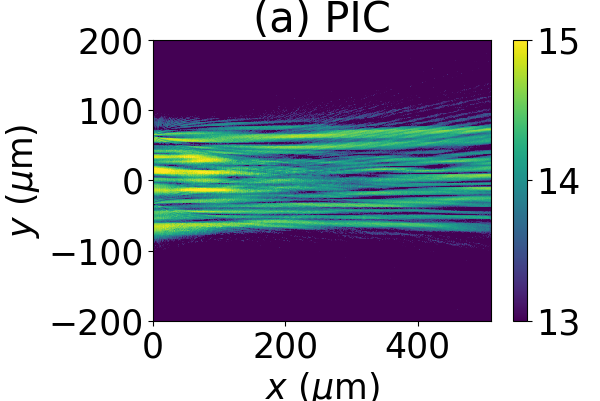
\includegraphics[scale=0.39]{Figure/I_Smilei24ps_te500eV_C6p.png}
&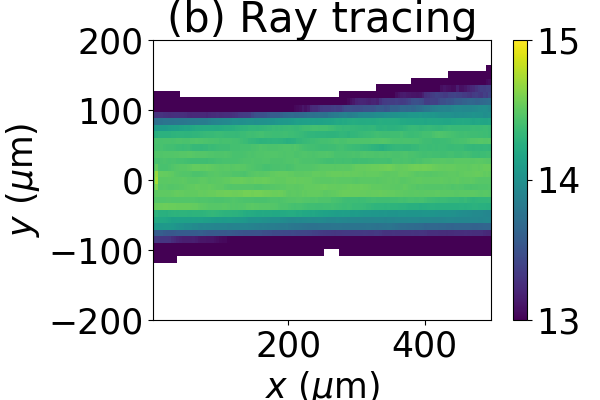
\includegraphics[scale=0.39]{Figure/I_HERA24ps_te500eV_C6p.png}
&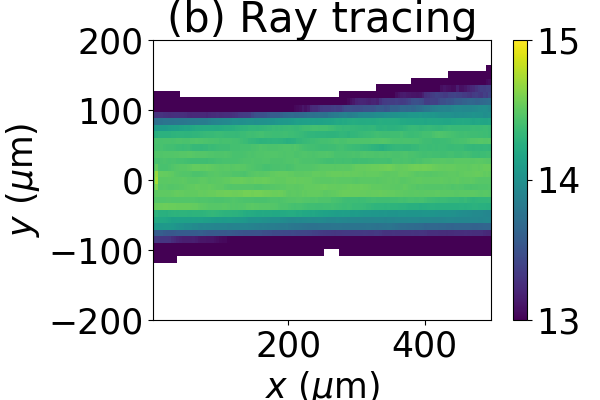
\includegraphics[scale=0.39]{Figure/I_HERA24ps_te500eV_C6p.png}\\
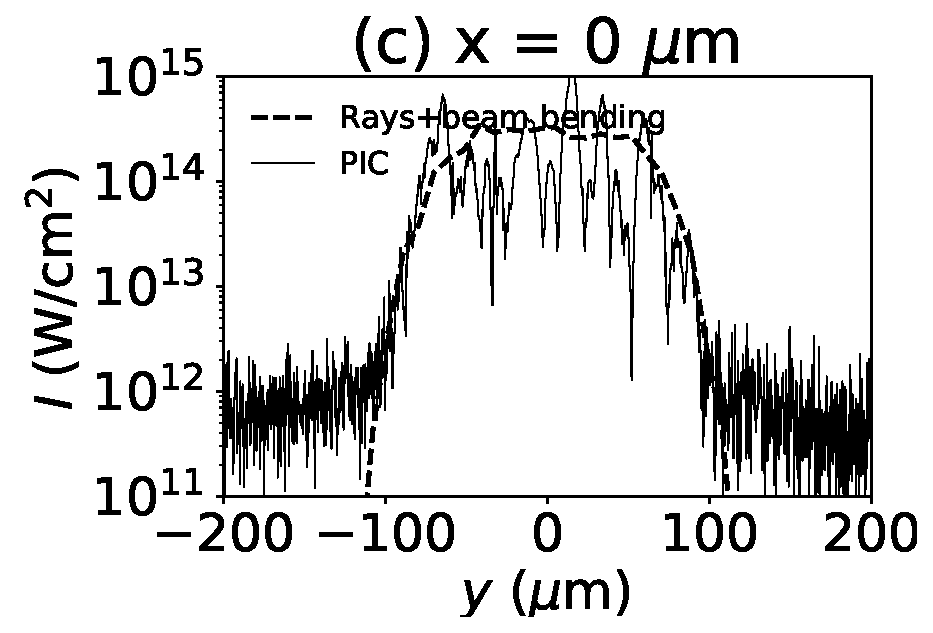
\includegraphics[scale=0.39]{Figure/Icut0_te500_C6p.eps}
&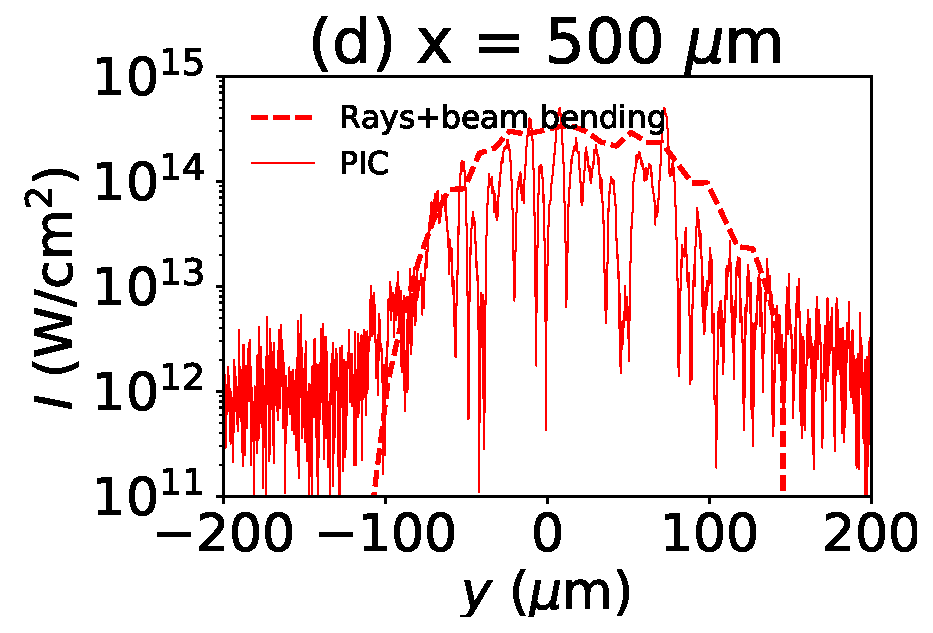
\includegraphics[scale=0.39]{Figure/Icut500_te500_C6p.eps}
&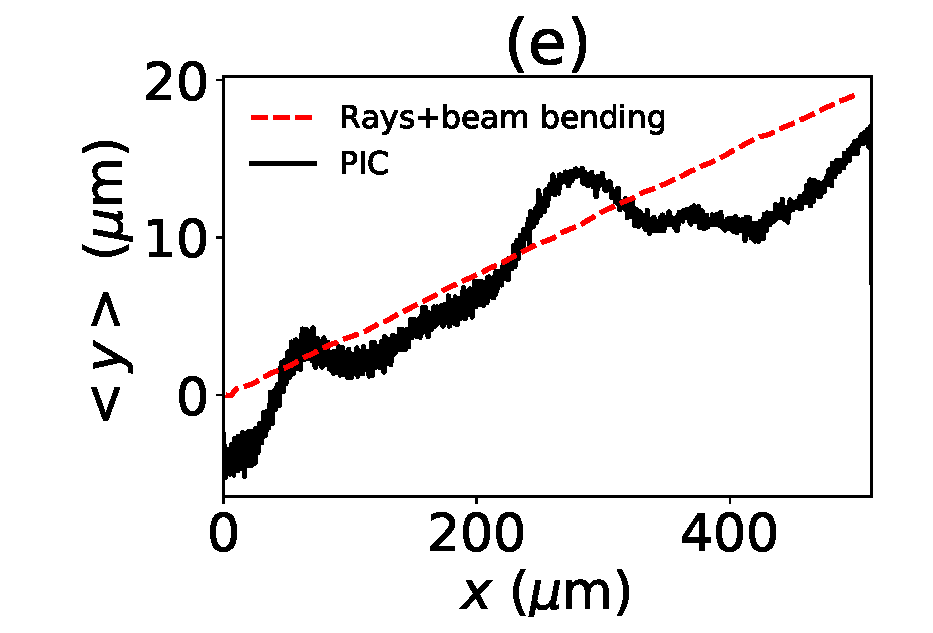
\includegraphics[scale=0.39]{Figure/ymoy_te500_C6p.eps}
\end{tabular}
\caption{ \label{fig:comthpicrpp} 
 Intensity in logscale at $t = 24$ ps of an RPP beam injected according to Eq. \eqref{eq:ebc} on the left boundary from a full PIC simulation (a), from hydrodynamics (HERA) with a paraxial propagation of the RPP beam including the correction of Eq. \eqref{eq:hydrof3} (b) and from the modified ray tracing model (c).  Lineout at $x=0$ (d) and $x=500 \, \rm \mu m$ (e) of   panel (a), (b) and (c). 
 (f) Centro\"id position (\emph{i.e.} the transverse position averaged over the intensity) from the PIC results (black solid line), from paraxial hydrodynamics (blue dashed) and  from the ray tracing scheme (red dashed line). The parameters of the C$^{6+}$ plasma are $n_e=0.1n_c$, $T_e=500$ eV, $T_i=3$ keV and $v_d=0.84 c_s$. }
\end{figure*}
\begin{figure*}
\begin{tabular}{ccc}
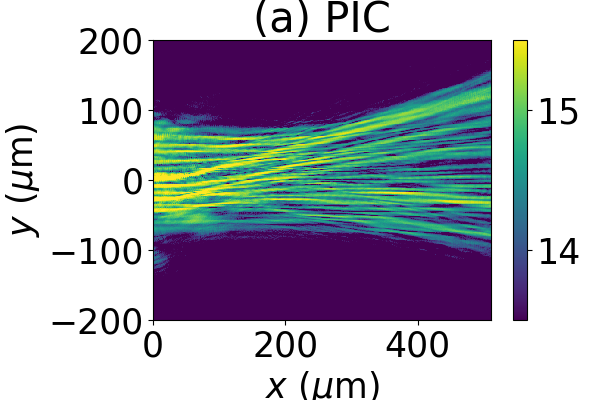
\includegraphics[scale=0.39]{Figure/I_Smilei18ps_te1keV_Ti1keV_.png}
&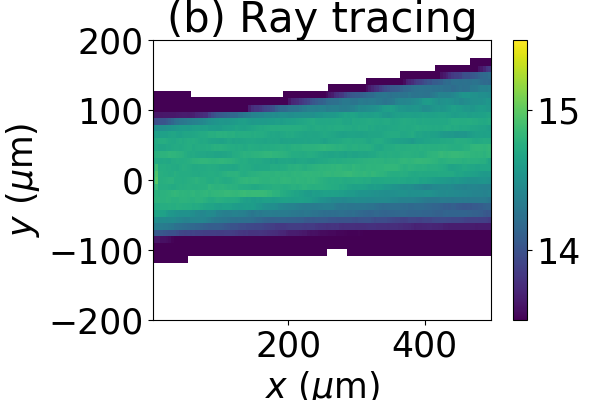
\includegraphics[scale=0.39]{Figure/I_HERA18ps_te1keV_Ti1keV_.png}
&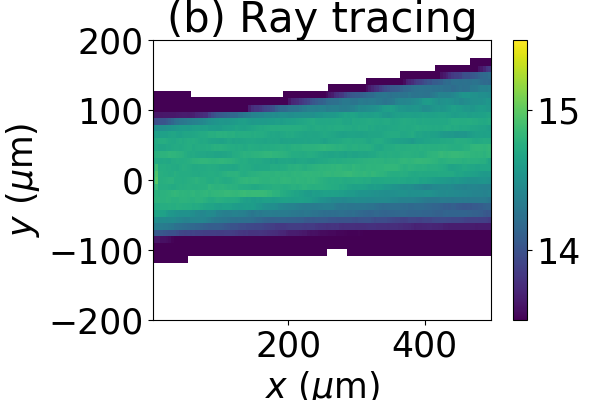
\includegraphics[scale=0.39]{Figure/I_HERA18ps_te1keV_Ti1keV_.png}\\
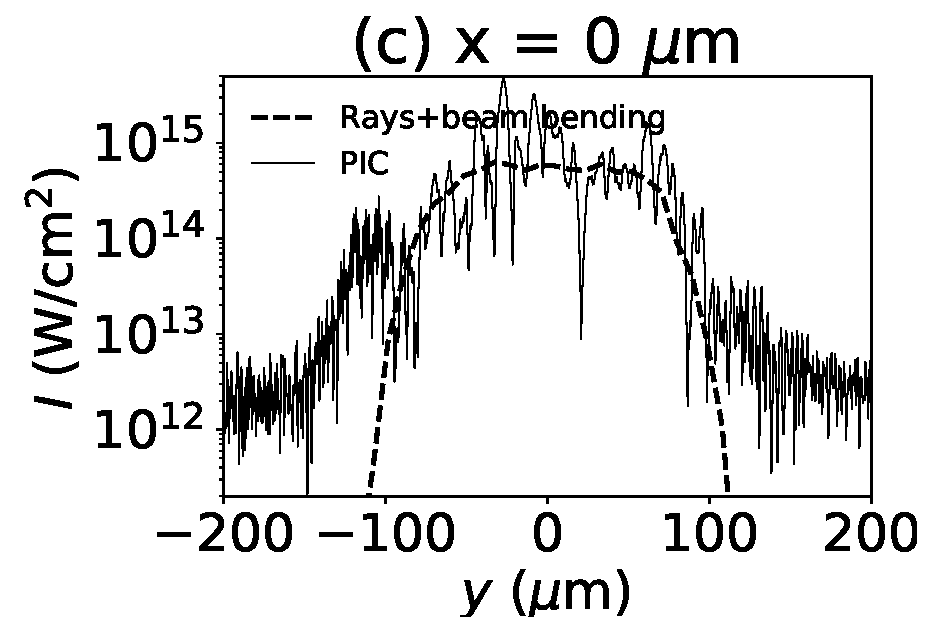
\includegraphics[scale=0.39]{Figure/Icut0_te1keV_Ti1keV_.eps}
&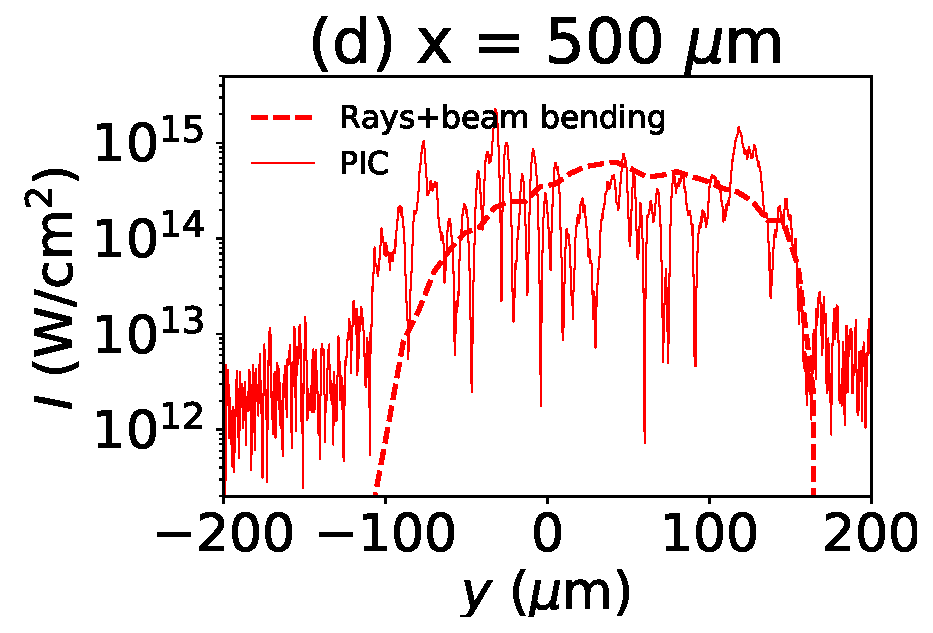
\includegraphics[scale=0.39]{Figure/Icut500_te1keV_Ti1keV_.eps}
&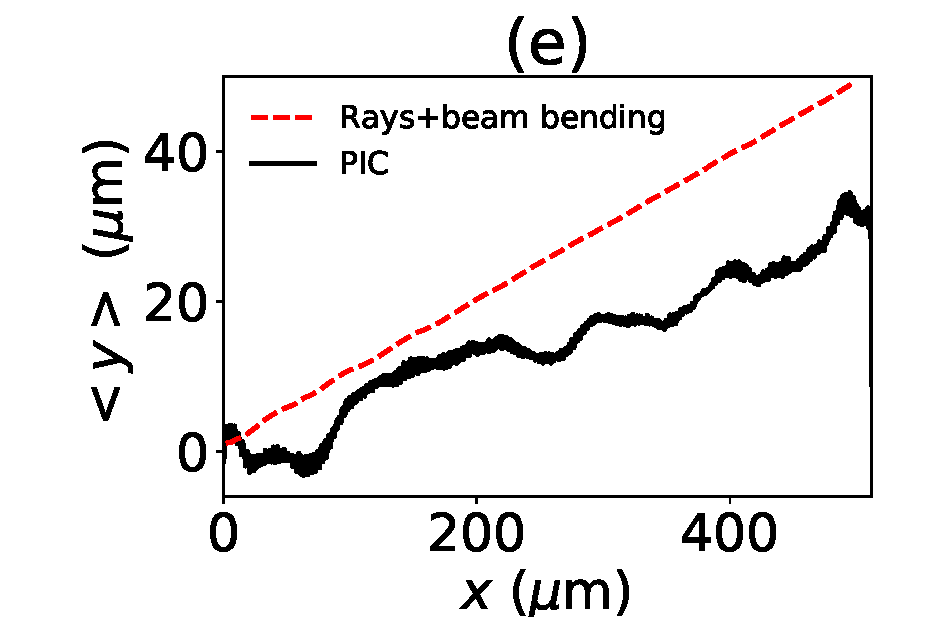
\includegraphics[scale=0.39]{Figure/ymoy_te1keV_Ti1keV_.eps}
\end{tabular}
\caption{ \label{fig:comthpicrpp2} 
Similar figures than in Fig. \ref{fig:comthpicrpp} for a H$^{+}$-plasma with $n_e=0.1n_c$, $T_e=1$ keV, $T_i=1$ keV, and $v_d=0.84 c_s$ at time $t= 18$ ps.  }
\end{figure*}
\begin{figure*}
\begin{tabular}{ccc}
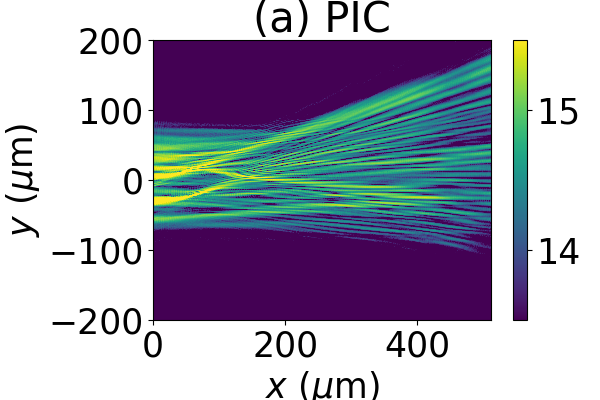
\includegraphics[scale=0.39]{Figure/I_Smilei20ps_te1keV_Ti300eV_.png}
&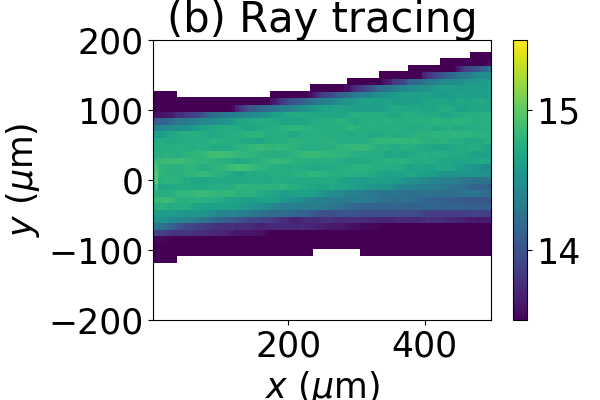
\includegraphics[scale=0.39]{Figure/I_HERA20ps_te1keV_Ti300eV_.png}
&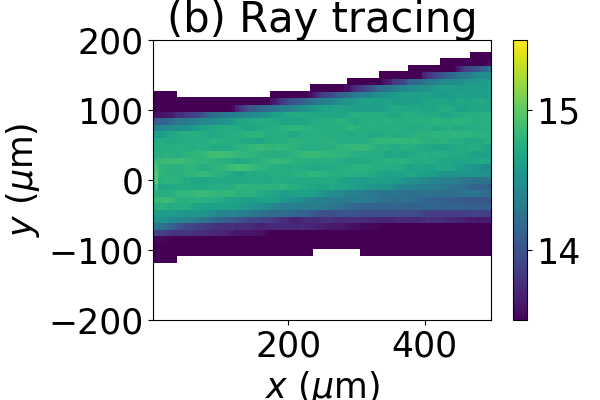
\includegraphics[scale=0.39]{Figure/I_HERA20ps_te1keV_Ti300eV_.png}\\
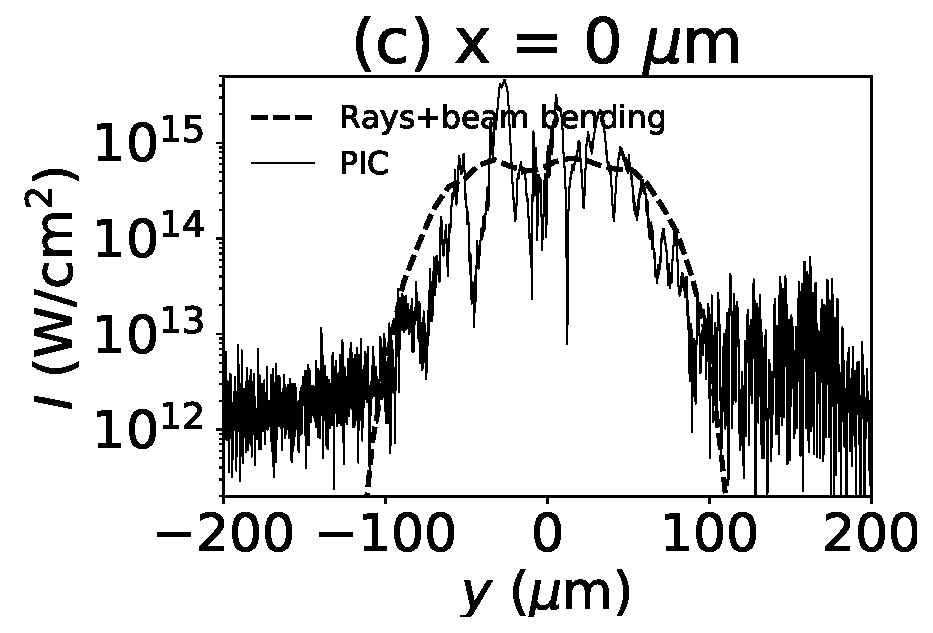
\includegraphics[scale=0.39]{Figure/Icut0_te1keV_Ti300eV_.eps}
&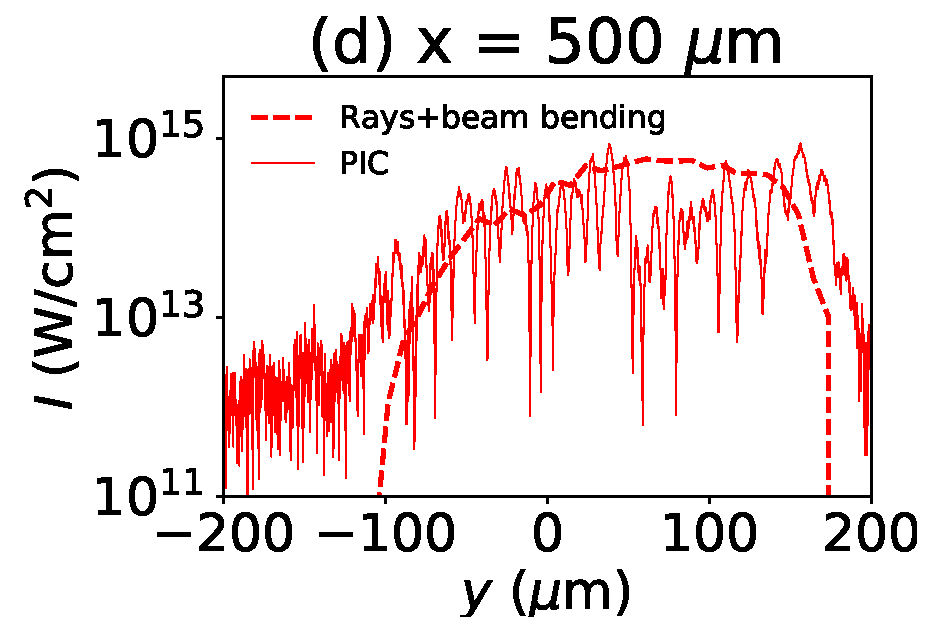
\includegraphics[scale=0.39]{Figure/Icut500_te1keV_Ti300eV_.eps}
&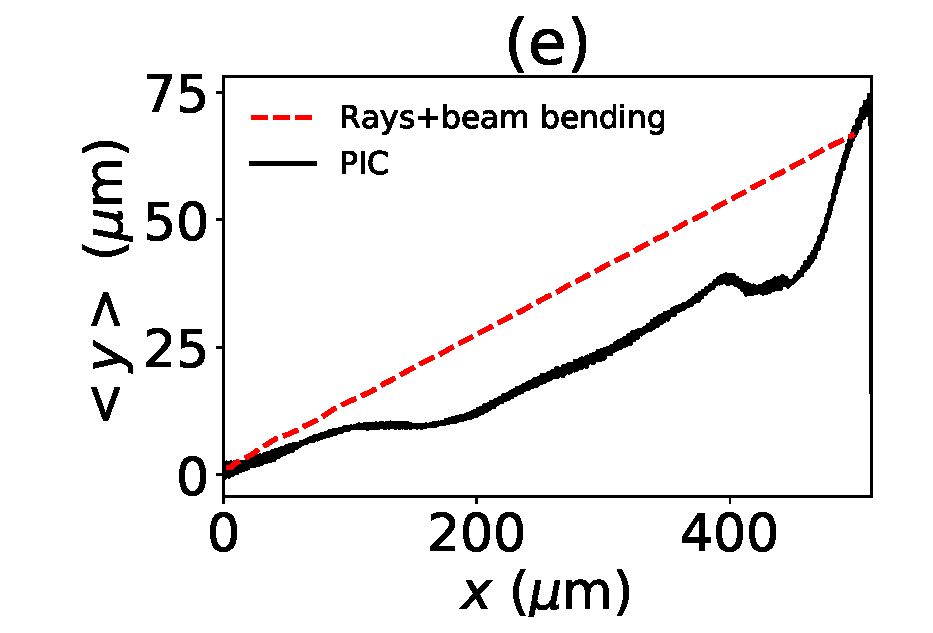
\includegraphics[scale=0.39]{Figure/ymoy_te1keV_Ti300eV_.eps}
\end{tabular}
\caption{ \label{fig:comthpicrpp3} 
Similar figures than in Fig. \ref{fig:comthpicrpp} for a  H$^{+}$-plasma with $n_e=0.1n_c$, $T_e=1$ keV, $T_i=300$ eV and $v_d=0.84 c_s$, at time $t = 20$ ps.
 \textcolor{red}{Mettre comparaison bin number et resolution}}
\end{figure*}

A quantitative comparison may now be carried between the  
exact solution obtained from large scale PIC simulations (with Smilei) and two types of  hydrodynamic simulations.
The first kind (HERA-ray) uses   HERA   with the modified ray tracing scheme (with large mesh size) and the second,  (HERA-parax) a paraxial solver (resolving the laser wavelength) for the RPP beam combined with the corrected ponderomove force introduced in Eqs. \eqref{eq:hydrof2}-\eqref{eq:hydrof3}. 

For all simulations codes, a 2D domain of size $L_x \times L_y = 512 \times 512\, \rm \mu$m$^2$ with the left boundary condition located at $x_\mathrm{BC}=0$ will be used. 
A RPP-beam (using Eqs. \eqref{eq:efoc} and  \eqref{eq:ebc}) or a ray tracing beam propagating in the $x$ direction were injected from the left boundary.
The focal spot is located at the center of the simulation domain, $x_\mathrm{foc}=256\, \rm \mu m$ with a speckle effective focal number of $f = 6.5$, a temporal
and spatial envelope following
\begin{align}
    \hat{g}(y) &= \exp(-\vert y\vert ^o/2\sigma_g^o)  \,  \\
    h(t) &= \mathrm{min}(t/\tau_h,1) \,
\end{align}
with a $\tau_h=1\, \rm ps$,  $o=5$ and $\sigma_g = 70\,\rm \mu m$. 
For sake of simplicity and comparison purposes, the bremsstrahlung energy deposition is neglected in HERA-ray and HERA-parax and does not occur in the collisionless PIC simulations.  Moreover perfect gaz is assumed in the hydrodynamics simulations.
As in Sec. \ref{sec:gauss}, all simulations in this study have been performed with $T_i \sim ZT_e$ in order to maximize the free-mode acoustic damping rate and therefore reduce as much as possible the stimulated Brillouin backward scattering. Moreover,  a total electron density of $n_e =0.1n_c $ is used  and a $y$-aligned drift velocity, $v_y=v_d$, is imposed on both the electron and ion populations.


Regarding the PIC simulations,  fully periodic boundary  conditions in the $y$ boundaries are applied for both fields and particles. Silver-M\"uller absorbent for the field and \textcolor{red}{absorbent} for the particles are used in the $x$ boundaries.  
A fourth order interpolation scheme is used with 36 particles per mesh per species, 21 points per laser wavelength and 14 points per laser temporal period. The plasma density is constant everywhere except on 12 microns close to both $x$ boundaries so that the effective plasma length is $0.488$  mm.

Regarding HERA-parax, use has been made of $dx =\lambda_0$, $dy = 0.125\lambda_0$ and $dt=10^{-13}$ s, \textcolor{red}{BC !}. 

In all two dimensional HERA-ray simulations shown in this study, the Cartesian grid has a mesh size of $dx=3.91\lambda_0$, $dy=9.37\lambda_0$ and $dt=5\times 10^{-13}$ s , much larger than the laser wavelength. The ray schemes use $10^4$ rays with regular speckle intensity bundles of width $dI/\langle I \rangle=0.1$ ranging from $I_\mathrm{max}/\langle I \rangle=2$ to $I_\mathrm{min}/\langle I \rangle=10$. \textcolor{red}{BC !}. 

The beam bending rate has been validated with three sets of parameters, namely a C$^{6+}$ plasma with $(T_e, T_i )= (500\, $eV$, 3\, $keV$)$ with an averaged laser intensity of $I_0 = 3\times 10^{14}\,\rm W.cm^{2}$, and a H$^{+}$ plasma  with $(T_e, T_i )= (1\, $keV$, 1 \,$keV$)$ and $(T_e, T_i )= (1\, $keV$, 300 \,$ eV$)$ with $I_0 = 6 \times 10^{14}\,\rm W.cm^{2}$.
Figs. \ref{fig:comthpicrpp}(a), \ref{fig:comthpicrpp2}(a) and \ref{fig:comthpicrpp3}(a) present the three aforementioned PIC simulations. All simulations unravel the deflection off its original course of a significant portion of the pulse energy  due to the beam bending effect.  
Very similar intensity profiles are obtained by the HERA-parax simulations illustrated in Figs. \ref{fig:comthpicrpp}(b), \ref{fig:comthpicrpp2}(b) and \ref{fig:comthpicrpp3}(b).
The ray tracing HERA-ray simulations [see Figs. \ref{fig:comthpicrpp}(c), \ref{fig:comthpicrpp2}(c) and \ref{fig:comthpicrpp3}(c)], although far less numerically constraining and neglecting the speckle-scale intensity fluctuations,   share a similar behavior than the PIC and HERA-parax simulations, \emph{i.e} more deflected light in the $y>100\,\rm\mu m$-region in the case of the H$^{+}$ than in the C$^{6+}$ plasma. 
All Smilei and HERA simulations evidence that the bending starts to affect the intensity profile for $x>200\,\rm\mu m$ for the H$^{+}$ case and  $x>300\,\rm\mu m$ for the C$^{6+}$.
\textcolor{red}{
The comparison of the intensity profiles  in Figs. \ref{fig:comthpicrpp}(c,d), \ref{fig:comthpicrpp2}(c,d) and \ref{fig:comthpicrpp3}(c,d) at $x=0$ and $500\,\rm\mu m$ illustrate the self-consistent description of the speckle scale field fluctuation in the PIC simulations (black solid lines). By contrast, the ray tracing scheme which only reproduces the averaged intensity fluctuations (red dashed lines), yield} much smoother profiles.
The laser centro\"ids, $\langle y \rangle$ [see Figs. \ref{fig:comthpicrpp}(e), \ref{fig:comthpicrpp2}(e) and \ref{fig:comthpicrpp3}(e)], measured in the PIC simulations by averaging the transverse position $y$ along the intensity transverse profile, exhibit some fluctuations. This tendency is probably due to the relatively weak number of speckle in our $\sim 70\,\rm\mu m$-focal spot, constrained by the high numerical cost of the kinetic simulations. 
The model satisfactorily captures the effect of the speckle-scale beam bending on the deflection of the averaged intensity envelope after $500\,\rm\mu m$ of propagation. 

The cases of Figs.  \ref{fig:comthpicrpp} (C$^{6+}$-plasma, $T_e=500$ eV) and Figs.  \ref{fig:comthpicrpp2} (H$^{+}$-plasma, $T_e=1$ keV)  correspond to the same values of $\delta n /n =0.031 $ and $ZT_e/T_i=1$, and therefore to the same asymptotic beam-bending rate [see Eq. \eqref{eq:dthf}]. However, Figs. \ref{fig:comthpicrpp}(a,b) present qualitatively much less deflection than in Figs. \ref{fig:comthpicrpp2}(a,b). The beam centro\"ids are shifted by $\sim 15\, \rm \mu m$ and  $\sim 40 \, \rm \mu m$ at $x=500 \, \rm \mu m$ in the C$^{6+}$  and H$^{+}$-plasma respectively [see Figs. \ref{fig:comthpicrpp}(c) and \ref{fig:comthpicrpp2}(c)].
This difference is caused by the larger temperature and therefore a shorter transient regime for the  H$^{+}$ plasma ($T_e=1$ keV, $t_0=10.5\, \rm ps$, Eq. \eqref{eq:t0}) than for the C$^{6+}$ one ($T_e=500$ eV, $t_0=21\, \rm ps$).
Hence the case of Fig. \ref{fig:comthpicrpp} is closer to the asymptotic limit and have a larger deflection angle per speckle than the case of Fig. \ref{fig:comthpicrpp2}. Such transient effects, negligible after a few tens of picoseconds of propagation of an RPP beam, is  of great importance  for understanding quantitatively the bending of temporally smoothed beams as shown subsequently.

The two sets of H$^+$-plasma simulations in   Figs. \ref{fig:comthpicrpp2} and  \ref{fig:comthpicrpp3}, 
differ only from their ions temperature, $T_i = 1000$ and $300 \, \rm eV$ respectively, giving  $\Im(\alpha_\mathrm{kin})=0.57$ and $2.59$ [see Eq. \eqref{eq:drakef}]. The driven acoustic damping rate is therefore smaller for  $T_i = 1000\, \rm eV$ than for  $300 \, \rm eV$ causing a weaker beam deflection, consistently with the line-outs at $500\,\rm \mu m$ which evidence less ledging at $y\gtrsim 100\,\rm\mu m$ and more depletion around $x\lesssim -50\,\rm\mu m$ in Fig. \ref{fig:comthpicrpp2}(c) than in  Fig. \ref{fig:comthpicrpp3}(c),  respectively. 

\textcolor{red}{Influence of the bundle number}

\section{Conclusions and prospects}

We revisited in this study the beam bending physics and shown that accounting for the accurate Landau damping of driven acoustic waves is crucial in order to  quantitatively capture the propagation of Gaussian laser pulse in a flowing plasma. 
In good agreement with dedicated PIC simulations, our bending rates analytical predictions allows the enhancement of ray tracing schemes relevant for nanoseconds and millimeter-scale hydrodynamic simulation of plasma and high-density matter  physics. We also introduced  a correction to the ponderomotive force which  accounts, in a fluid code, for the influence of kinetic driven acoustic wave damping on the density fluctuations and the resulting light propagation. 

We then demonstrated that both the ponderomotive correction and the modified ray tracing schemes correctly capture the centro\"id deviation and the amount of scattered light of an RPP beam propagating in a flowing plasma. Hence, the speckle-scale physics of crucial importance for many wave-mixing processes, may be included in coarse description of light such as  ray tracing-based schemes. 

Note that, although out of the scope of this study, the generalisation to three dimensions of the modified ray tracing scheme seems feasible. Na\"ively, in addition to deriving the main equations in three dimensions, one would only have to use the speckle abundance formulas in realistic geometry in order to accurately capture the speckle-scale bending of a RPP  pulse. 
Moreover, temporal  smoothing techniques is known to reduce the beam bending as it introduces a finite speckle coherence time of the order of a few picoseconds. The generalization of our model to three dimension and to the  modeling of SSD beams is left for future work, along with its interplay with other wave-mixing processes.

\section*{Acknowledgements}
We acknowledge fruitful discussions with the  Smilei-team, particurlarly  F. Perez, M. Grech, A. Beck and J. Derouillat.
 \textcolor{red}{We also acknowledge D. Dureau and the HERA-team for all their work on the HERA code. }
This work has been done under  the auspices of  CEA-DAM and
the simulations were performed using HPC resources at TGCC/CCRT and CEA-DAM/TERA.
\bibliography{biblio}
\end{document}
